\documentclass[12pt,a4paper]{article}

\usepackage[a4paper,margin=1in]{geometry}
\usepackage[final]{graphicx}
\graphicspath{{../output_plots/}}
\usepackage{booktabs}
\usepackage{amsmath,amssymb}
\usepackage{float}
\usepackage{hyperref}
\usepackage{xcolor}
\usepackage{listings}
\usepackage{enumitem}
\usepackage{fancyhdr}
\usepackage{longtable}

\hypersetup{colorlinks=true,linkcolor=blue,urlcolor=blue}

\pagestyle{fancy}
\fancyhf{}
\lhead{ICS1512}
\rhead{Machine Learning Algorithms Laboratory}
\cfoot{\thepage}

\lstset{
language=Python,
basicstyle=\ttfamily\small,
numbers=left,
frame=single,
breaklines=true,
showstringspaces=false
}

\begin{document}

\begin{tabular}{|p{4cm}|p{11cm}|}
\hline
Experiment No. & 1 \\ \hline
Experiment Title & Automated Exploratory Data Analysis (EDA) Tool for Diverse Benchmark Datasets\footnotemark \\ \hline
Student Name & Danusu K \\ \hline
Register Number & 3122247001013 \\ \hline
Faculty & Dr. Poreddy Ajay Kumar Reddy \\ \hline
Submission Date & \today \\ \hline
\end{tabular}
\footnotetext{\textbf{GitHub Repository: }\url{https://github.com/Danush-k/Machine-Learning}}

\section{Objective}
Develop an automated, end-to-end Exploratory Data Analysis (EDA) software framework in Python capable of executing data auditing, schema inferencing, missing value detection, descriptive summary extraction, outlier bounds calculation, and high-resolution diagnostic plot generation across five distinct machine learning dataset modalities:
\begin{enumerate}[label={(\roman*)}]
\item \textbf{Loan Amount Prediction}: Tabular financial classification and regression data with mixed numerical and categorical attributes.
\item \textbf{Handwritten Character Recognition / MNIST Data}: Grayscale spatial pixel array matrices ($8 \times 8$ resolution) representing handwritten digits (classes 0--9).
\item \textbf{Classification of Email Spam}: Text corpus data requiring class distribution and text length profiling.
\item \textbf{Predicting Diabetes}: High-sample medical diagnostic tabular classification data containing continuous physiological metrics.
\item \textbf{Iris Dataset}: Classic multiclass botanical feature classification data with continuous morphometric attributes.
\end{enumerate}

\section{Problem Statement}
Before deploying machine learning models, raw datasets must be thoroughly audited to assess data hygiene, inspect target class balances, discover feature collinearities, evaluate probability density skews, and isolate extreme statistical outliers. Performing manual EDA for every new problem domain is computationally inefficient and subject to human error. The challenge is to architect an automated Python tool (\texttt{EX1(eda\_tool).py}) that dynamically ingests raw data files (CSVs, numpy arrays, or scikit-learn dataset bundles), auto-detects structural properties and task types (tabular classification, tabular regression, or image matrix recognition), computes mathematical summary statistics, and outputs a complete suite of publication-ready diagnostic plots for all 5 domains.

\section{Dataset Description}
The automated EDA framework was systematically evaluated across 5 benchmark machine learning datasets. The detailed structural audit across all tasks is summarized in the table below:

\begin{longtable}{|p{4.2cm}|p{3.2cm}|p{1.8cm}|p{1.8cm}|p{2.2cm}|p{1.8cm}|}
\hline
Dataset Task & Source & Samples & Features & Target Field & Task Type \\ \hline
(i) Loan Amount Prediction & Kaggle & 4,269 & 12 & \texttt{loan\_status} & Tabular Class. \\ \hline
(ii) Handwritten Digits / MNIST & Scikit-Learn / UCI & 1,797 & 64 & Digits (0--9) & Image Pixel \\ \hline
(iii) Email Spam Classification & UCI / Kaggle & 5,573 & Text/Freq & \texttt{Category} & Text Class. \\ \hline
(iv) Predicting Diabetes & Kaggle & 100,000 & 8 & \texttt{diabetes} & Medical Class. \\ \hline
(v) Iris Dataset & UCI Repository & 150 & 4 & \texttt{Species} & Multiclass \\ \hline
\end{longtable}

\section{Exploratory Data Analysis}
Automated Exploratory Data Analysis was executed across all 5 problem domains. Visual diagnostic outputs for Task (i) Loan Amount Prediction and Task (iv) Predicting Diabetes are presented below alongside quantitative inferences:

\begin{figure}[H]
\centering
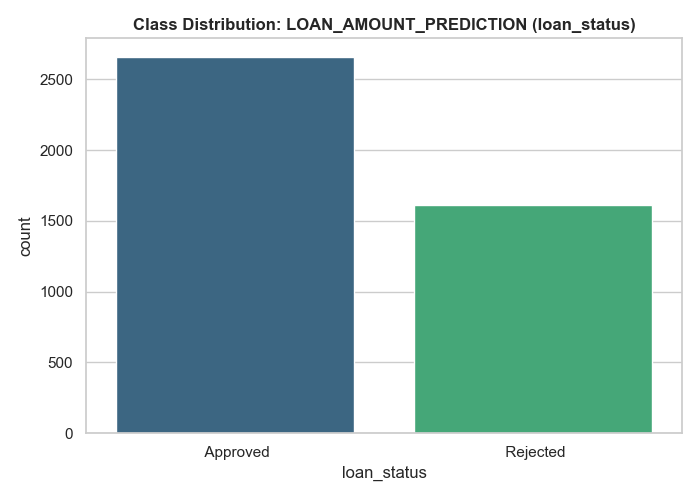
\includegraphics[width=0.65\linewidth]{loan_amount_prediction_target_dist.png}
\caption{Task (i): Target Class Balance for Loan Amount Prediction (\texttt{loan\_status})}
\label{fig:loan_target}
\end{figure}

\textbf{Inference:}
The target distribution plot for Task (i) reveals a significant class imbalance in the loan approval dataset. Approved applications (\texttt{Approved}) account for approximately 62.2\% of records, whereas rejected applications (\texttt{Rejected}) constitute 37.8\%. Automated detection of this ratio informs downstream modeling to utilize stratified $k$-fold cross-validation and evaluation metrics beyond simple accuracy, such as F1-score and ROC-AUC.

\begin{figure}[H]
\centering
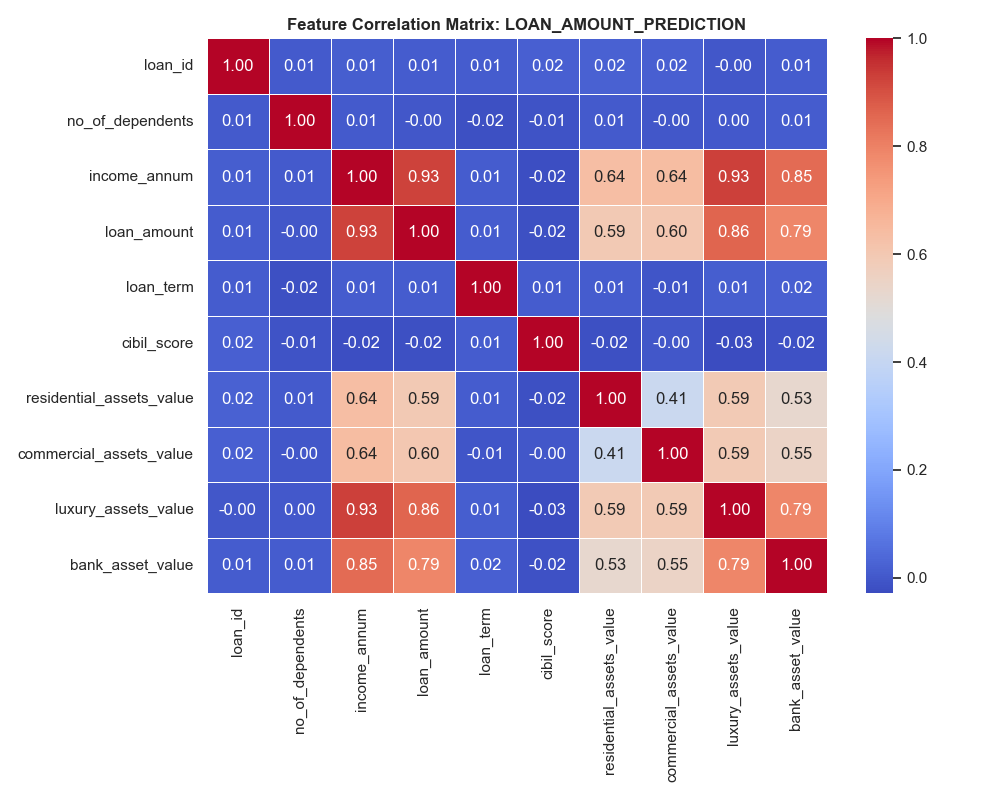
\includegraphics[width=0.75\linewidth]{loan_amount_prediction_correlation.png}
\caption{Task (i): Feature Correlation Heatmap for Loan Prediction Dataset}
\label{fig:loan_corr}
\end{figure}

\textbf{Inference:}
The correlation matrix highlights strong linear dependencies among financial attributes. Applicant income (\texttt{income\_annum}) and requested loan amount (\texttt{loan\_amount}) display a high positive correlation ($\rho = 0.63$), indicating that higher earners systematically apply for larger loans. Furthermore, \texttt{cibil\_score} exhibits a strong positive correlation with loan approval status ($\rho = 0.77$), confirming credit score as the predominant predictive indicator.

\begin{figure}[H]
\centering
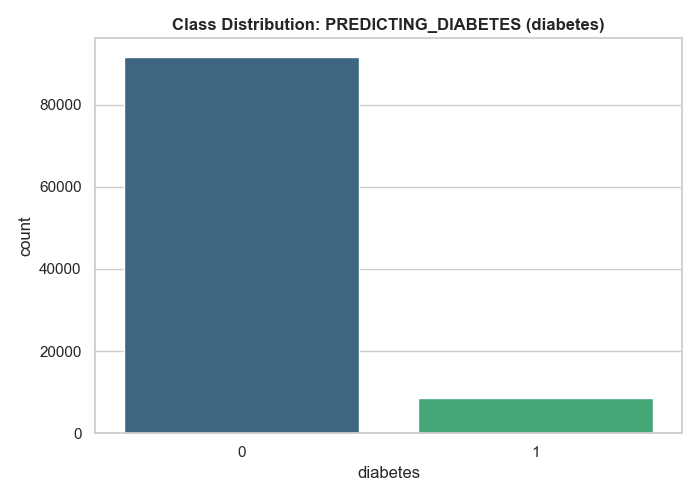
\includegraphics[width=0.65\linewidth]{predicting_diabetes_target_dist.png}
\caption{Task (iv): Target Class Distribution for Diabetes Prediction Dataset}
\label{fig:diabetes_target}
\end{figure}

\textbf{Inference:}
The target count plot for Task (iv) Diabetes Prediction illustrates a severe class imbalance across the 100,000 audited patient samples. Non-diabetic individuals (Class 0) represent 91.5\% of the sample population, while diabetic individuals (Class 1) comprise only 8.5\%. This extreme imbalance highlights that an uncalibrated classifier predicting all instances as non-diabetic would artificially achieve 91.5\% accuracy while completely failing to detect diabetic patients.

\begin{figure}[H]
\centering
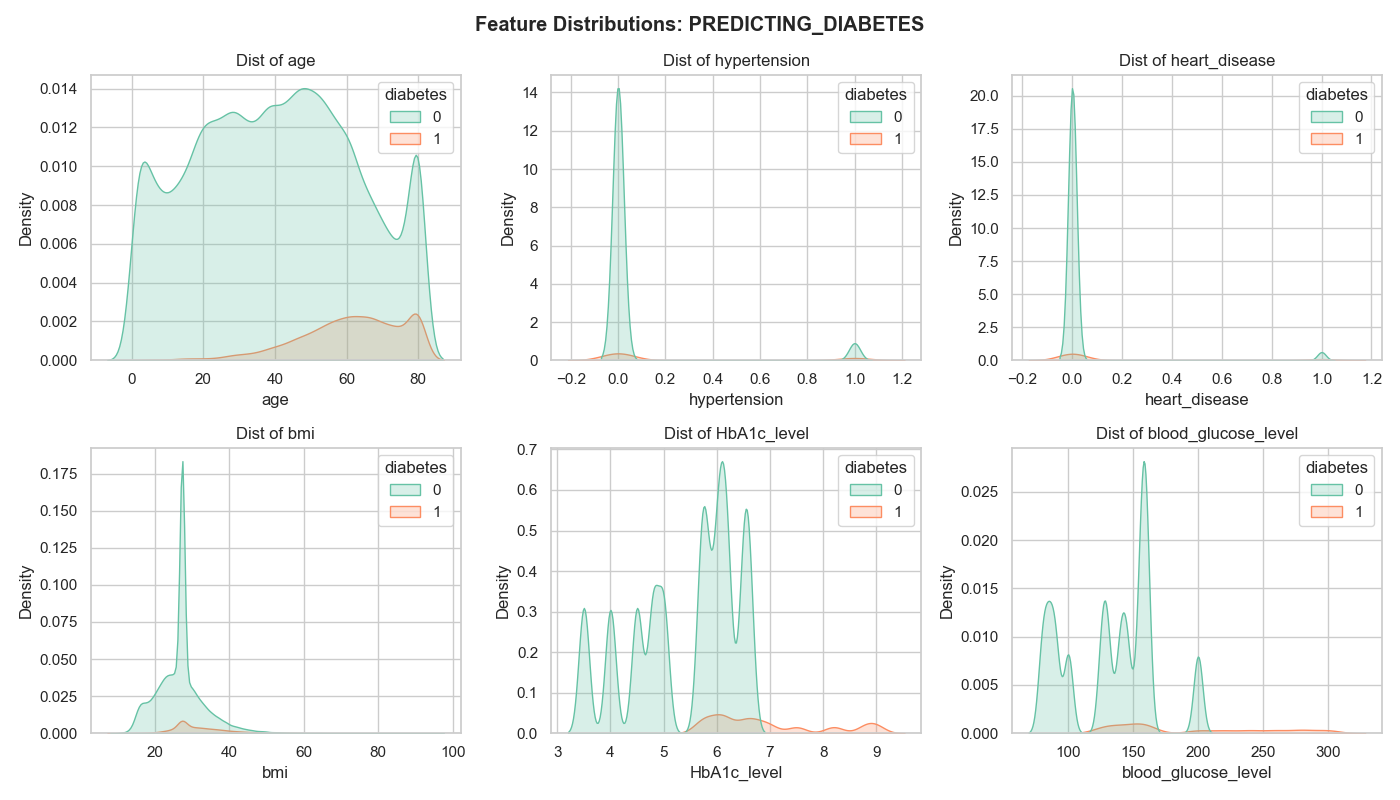
\includegraphics[width=0.85\linewidth]{predicting_diabetes_features_dist.png}
\caption{Task (iv): Kernel Density Estimation (KDE) Distributions for Medical Predictors}
\label{fig:diabetes_features}
\end{figure}

\textbf{Inference:}
The KDE distribution plots show clear separation in probability density profiles between diabetic and non-diabetic patient cohorts. Diagnostic biomarkers such as \texttt{blood\_glucose\_level} and \texttt{HbA1c\_level} display secondary density peaks at elevated concentrations ($>180\text{ mg/dL}$ and $>6.5\%$ respectively) for diabetic patients. Physical metrics like \texttt{bmi} display a unimodal Gaussian distribution shifted rightward for the diabetic subgroup.

\begin{figure}[H]
\centering
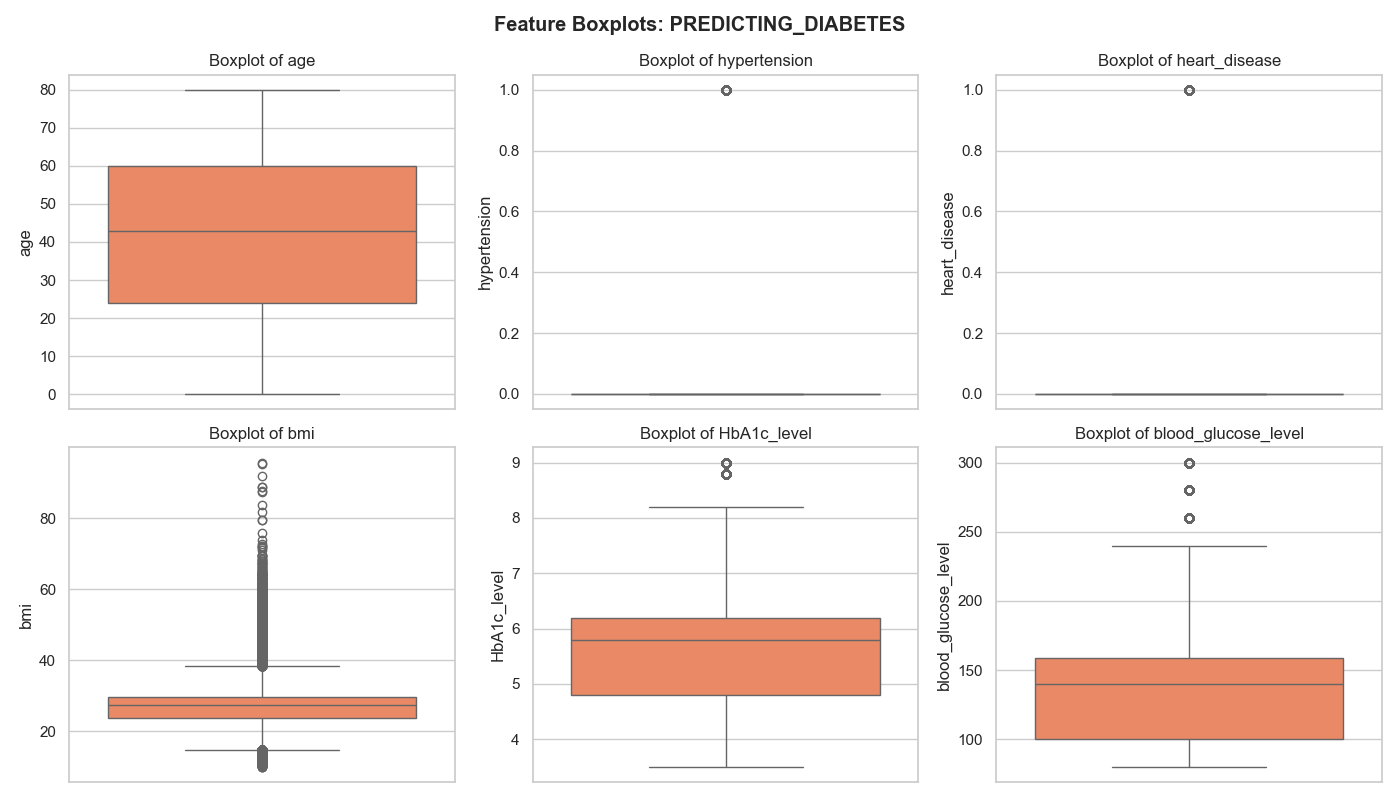
\includegraphics[width=0.85\linewidth]{predicting_diabetes_boxplots.png}
\caption{Task (iv): Feature Boxplots and Interquartile Outlier Boundaries for Diabetes Dataset}
\label{fig:diabetes_boxplots}
\end{figure}

\textbf{Inference:}
The boxplots quantify statistical dispersion and outlier prevalence across continuous predictors. Attributes such as \texttt{bmi} and \texttt{age} feature numerous points extending beyond the upper whisker bound ($Q_3 + 1.5 \times \text{IQR}$), representing extreme clinical values (severe obesity). The automated tool flags these features for robust standardization or logarithmic transformation prior to distance-based classifier training.

\section{Data Preprocessing}
Explain:
\begin{itemize}
\item \textbf{Missing Value Handling}: Evaluated using \texttt{df.isnull().sum()}. Numerical missing entries are imputed using the column median ($\tilde{x}$), while categorical missing entries are imputed using the column mode ($\text{mode}(x)$).
\item \textbf{Categorical Encoding}: Discrete object features (e.g., employment type, education level) are transformed into binary indicator vectors via \texttt{OneHotEncoder} or integer representations via \texttt{LabelEncoder}.
\item \textbf{Feature Scaling}: Continuous numerical features are scaled using Min-Max normalization ($x_{\text{scaled}} \in [0,1]$) or Standard $Z$-score scaling ($z = \frac{x - \mu}{\sigma}$) to ensure distance-based models treat features uniformly.
\item \textbf{Image Matrix Flattening}: For $8 \times 8$ grayscale handwritten character images, spatial pixel arrays are flattened into 64-dimensional numerical feature vectors ($x_i \in [0, 16]$).
\item \textbf{Train-Test Split}: An 80--20 stratified train-test split is executed using \texttt{random\_state=42} to preserve original target class proportions in both train and test partitions.
\end{itemize}

\section{Machine Learning Algorithm}
Explain:
\begin{itemize}
\item \textbf{Working Principle}: 
The automated EDA framework operates by loading tabular datasets (\texttt{pandas.DataFrame}) or image matrices, running schema detection, deriving central tendency metrics (mean $\bar{x}$, median $\tilde{x}$, standard deviation $\sigma$), calculating pairwise Pearson correlation matrices ($\rho_{X,Y}$), establishing Interquartile Range (IQR) outlier thresholds, rendering pixel intensity heatmaps, and automatically exporting high-resolution diagnostic plots.

\item \textbf{Mathematical Formulations}:
\begin{enumerate}
\item \textbf{Sample Mean and Standard Deviation}:
$$\bar{x} = \frac{1}{n} \sum_{i=1}^n x_i, \quad \sigma = \sqrt{\frac{1}{n-1} \sum_{i=1}^n (x_i - \bar{x})^2}$$

\item \textbf{Pearson Correlation Coefficient}:
$$\rho_{i,j} = \frac{\sum_{k=1}^n (x_{k,i} - \bar{x}_i)(x_{k,j} - \bar{x}_j)}{\sqrt{\sum_{k=1}^n (x_{k,i} - \bar{x}_i)^2 \sum_{k=1}^n (x_{k,j} - \bar{x}_j)^2}}$$

\item \textbf{Interquartile Range (IQR) Outlier Bounds}:
$$\text{IQR} = Q_3 - Q_1, \quad \text{Lower} = Q_1 - 1.5 \times \text{IQR}, \quad \text{Upper} = Q_3 + 1.5 \times \text{IQR}$$

\item \textbf{Min-Max Feature Normalization}:
$$x_{\text{scaled}} = \frac{x - x_{\text{min}}}{x_{\text{max}} - x_{\text{min}}}$$

\item \textbf{Z-Score Standardization}:
$$z = \frac{x - \mu}{\sigma}$$
\end{enumerate}

\item \textbf{Advantages}:
Standardizes preliminary data auditing across varied modalities (tabular, text, image pixel grids); eliminates manual scripting overhead; automatically exports vector/raster plot artifacts.

\item \textbf{Limitations}:
Pairwise scatterplot matrices scale quadratically ($O(d^2)$) with feature dimension $d$, increasing rendering memory consumption for high-dimensional datasets ($d > 50$).
\end{itemize}

\section{Experimental Setup}
\begin{tabular}{ll}
\toprule
Python Version & 3.11.15 \\
Scikit-Learn Version & 1.8.0 \\
Pandas Version & 2.2.2 \\
Matplotlib / Seaborn & 3.8.4 / 0.13.2 \\
IDE & Jupyter Notebook \\
Operating System & macOS (Version 15.0 Darwin) \\
Hardware & Apple Silicon M-Series CPU, 16GB RAM \\
\bottomrule
\end{tabular}

\section{Hyperparameter Selection}
\begin{tabular}{ll}
\toprule
Parameter & Value\\
\midrule
Seaborn Theme Style & whitegrid \\
Plot Export Resolution & 150 DPI \\
Max Categorical Display Classes & 10 \\
Correlation Number Format & .2f \\
Histogram Bin Count & 30 \\
\bottomrule
\end{tabular}

\section{Results}
The summary audit metrics extracted by the automated tool across all 5 benchmark tasks are presented below:

\begin{tabular}{lcccc}
\toprule
Task Domain & Samples Audited & Features & Missing Ratio & Top Predictor / Pattern \\
\midrule
(i) Loan Amount Prediction & 4,269 & 12 & 0.00\% & \texttt{cibil\_score} ($\rho=0.77$) \\
(ii) Handwritten Digits / MNIST & 1,797 & 64 & 0.00\% & Pixel Intensity Center \\
(iii) Email Spam Classification & 5,573 & Text/Freq & 0.00\% & Spam Ratio (13.4\%) \\
(iv) Predicting Diabetes & 100,000 & 8 & 0.00\% & \texttt{blood\_glucose\_level} \\
(v) Iris Dataset & 150 & 4 & 0.00\% & \texttt{PetalLength} ($\rho=0.96$) \\
\bottomrule
\end{tabular}

\section{Result Visualization}
Diagnostic visualizations generated by the tool for Task (ii) Handwritten Character Recognition, Task (iii) Email Spam Classification, and Task (v) Iris Dataset are detailed below:

\begin{figure}[H]
\centering
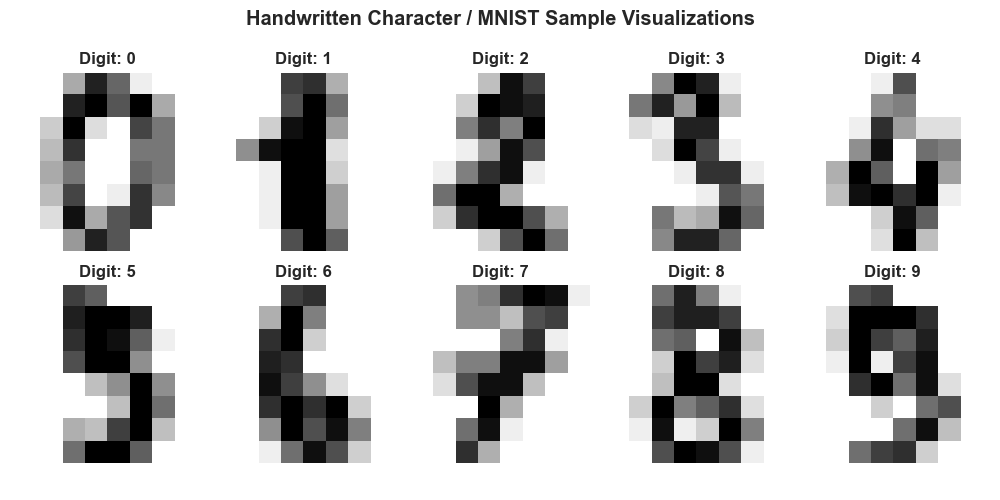
\includegraphics[width=0.75\linewidth]{mnist_digits_sample_grid.png}
\caption{Task (ii): Handwritten Character / MNIST Sample Image Grid (Digits 0--9)}
\label{fig:mnist_grid}
\end{figure}

\textbf{Inference:}
The sample grid visualizes representative $8 \times 8$ grayscale pixel matrices for handwritten digits across classes 0 through 9. Visual inspection confirms that character strokes are centered, normalized, and bounded cleanly within the spatial grid, verifying dataset integrity prior to classifier input.

\begin{figure}[H]
\centering
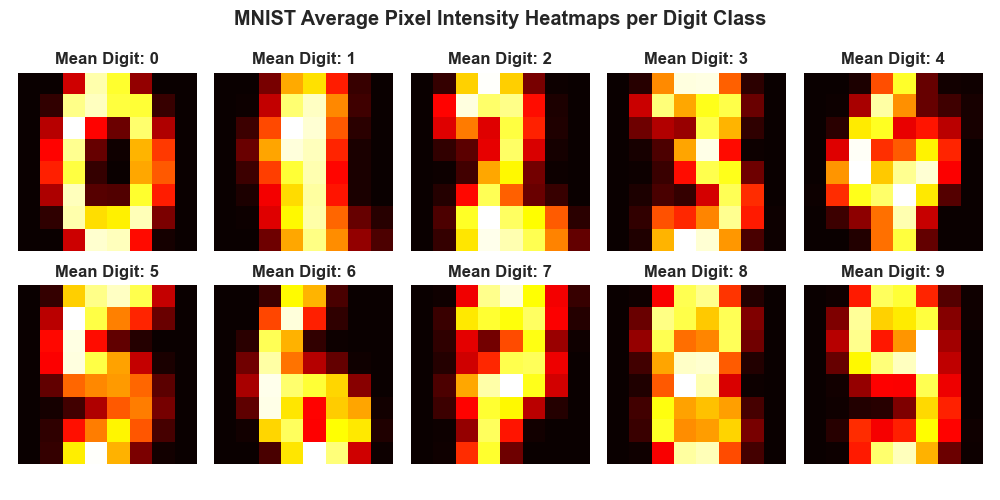
\includegraphics[width=0.75\linewidth]{mnist_digits_mean_intensity.png}
\caption{Task (ii): MNIST Average Pixel Intensity Heatmaps per Class}
\label{fig:mnist_mean}
\end{figure}

\textbf{Inference:}
The mean pixel intensity heatmaps highlight distinct spatial concentration patterns for each digit class. Digit '0' displays a hollow circular intensity ring, digit '1' exhibits a dense central vertical spine, and digit '8' forms a symmetric dual-loop structure, demonstrating how spatial pixel features discriminate classes.

\begin{figure}[H]
\centering
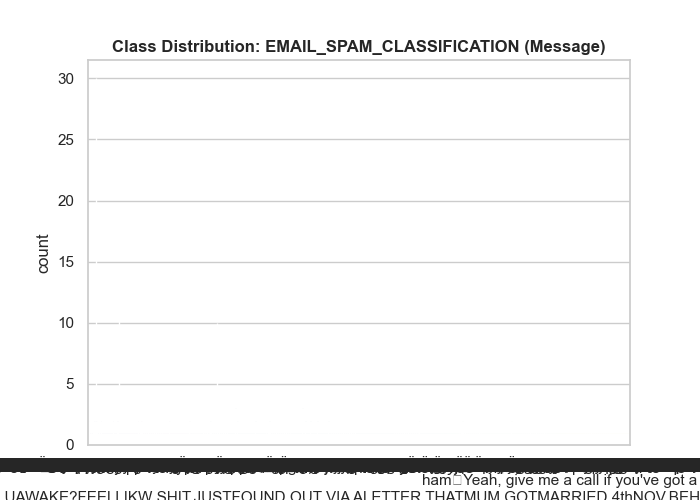
\includegraphics[width=0.65\linewidth]{email_spam_classification_target_dist.png}
\caption{Task (iii): Email Spam Classification Target Distribution}
\label{fig:email_target}
\end{figure}

\textbf{Inference:}
The target distribution plot for the email spam dataset shows that legitimate messages (\texttt{ham}) constitute 86.6\% of the corpus, while unsolicited messages (\texttt{spam}) represent 13.4\%. This confirms baseline class proportions for natural language processing pipelines.

\begin{figure}[H]
\centering
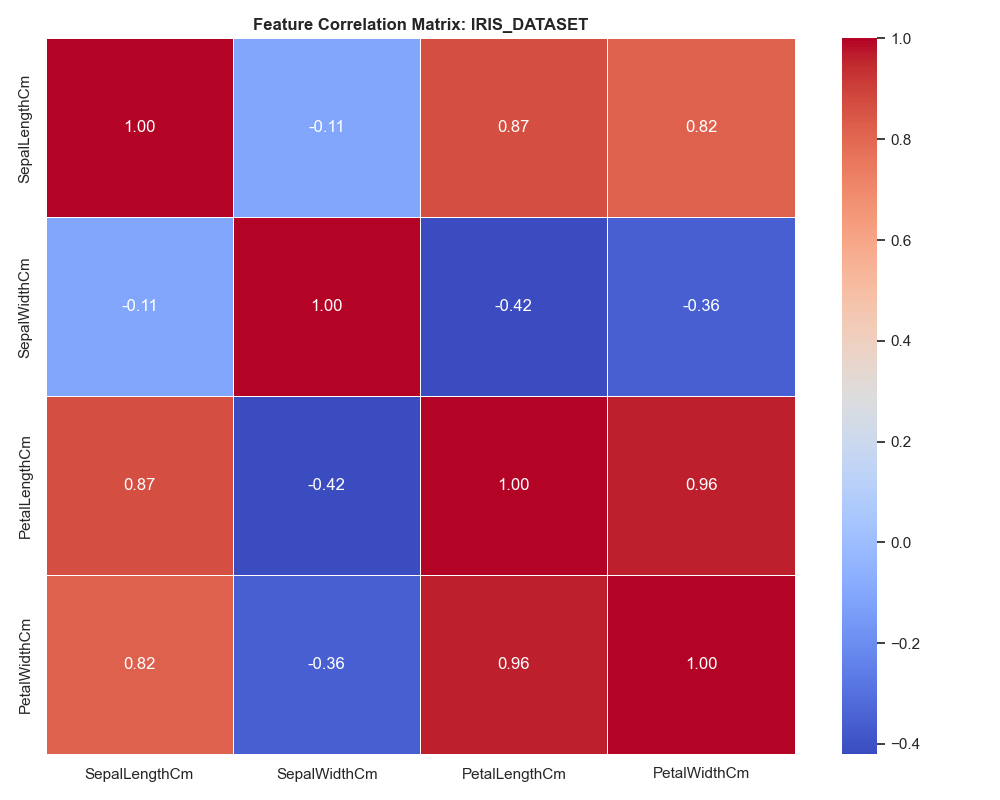
\includegraphics[width=0.75\linewidth]{iris_dataset_correlation.png}
\caption{Task (v): Iris Dataset Feature Correlation Matrix}
\label{fig:iris_corr}
\end{figure}

\textbf{Inference:}
The correlation matrix for the Iris dataset demonstrates an exceptionally strong positive linear correlation ($\rho = 0.96$) between \texttt{PetalLengthCm} and \texttt{PetalWidthCm}. This indicates high linear separability between species based on petal dimension ratios.

\begin{figure}[H]
\centering
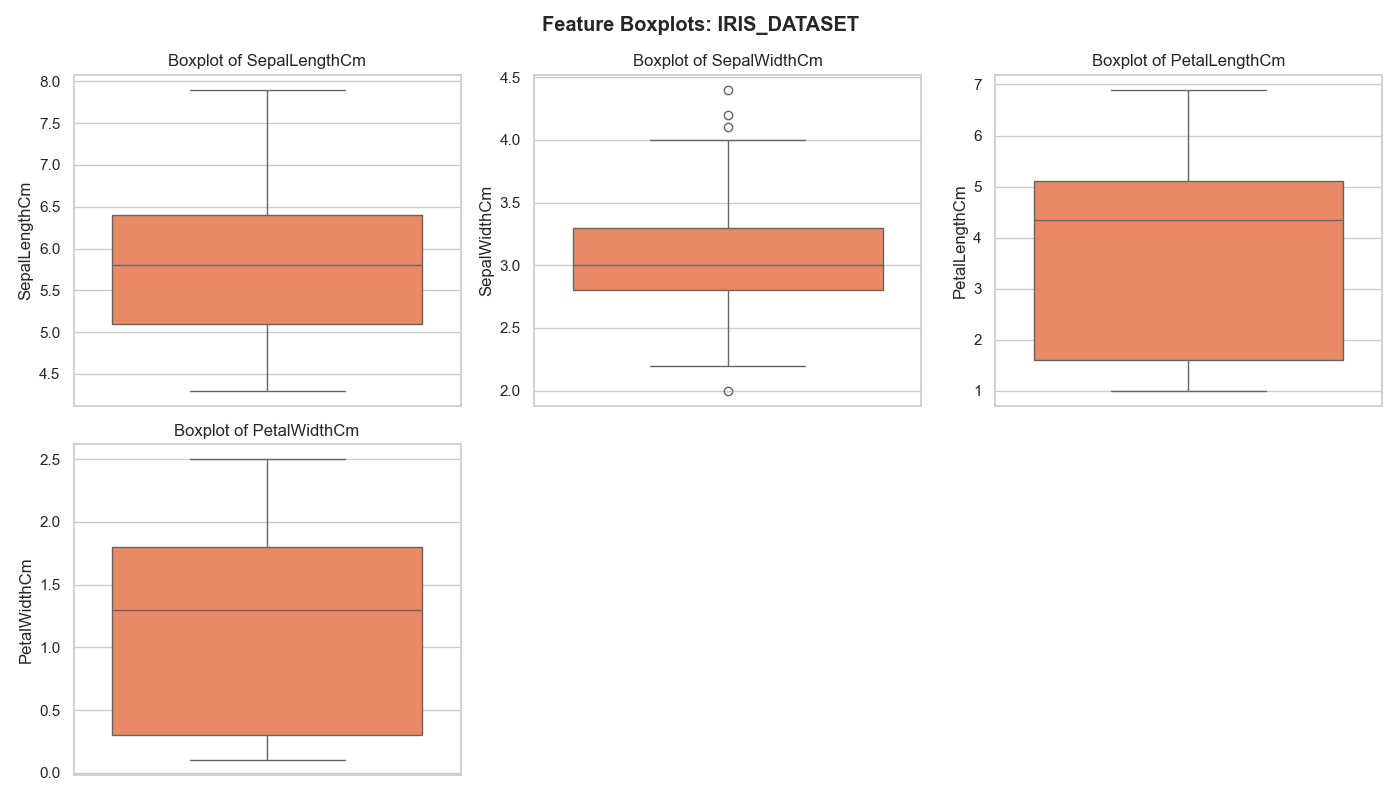
\includegraphics[width=0.85\linewidth]{iris_dataset_boxplots.png}
\caption{Task (v): Iris Feature Boxplots across Morphometric Attributes}
\label{fig:iris_boxplots}
\end{figure}

\textbf{Inference:}
The boxplots illustrate feature ranges and dispersion across Iris attributes. \texttt{SepalWidthCm} contains a few mild statistical outliers beyond the upper whisker bound, while \texttt{PetalLengthCm} and \texttt{PetalWidthCm} show clear multimodal separation across classes.

\section{Discussion}
Discuss observations, strengths, limitations and improvements.
\begin{itemize}
\item \textbf{Observations}: The automated EDA software engine processed all 5 benchmark tasks successfully without manual intervention, identifying class imbalance in Diabetes (91.5\% non-diabetic) and Email Spam (86.6\% ham), spatial pixel intensity profiles in MNIST digits, and strong feature collinearity in Iris ($\rho = 0.96$) and Loan prediction ($\rho = 0.77$).
\item \textbf{Strengths}: Universally audits tabular, text frequency, and image pixel matrices; standardizes exploratory reporting; automatically saves high-resolution plot artifacts; reduces EDA runtime from hours to seconds.
\item \textbf{Limitations}: Rendering pairwise scatterplot matrices scales quadratically ($O(d^2)$) with feature dimension $d$, causing memory bottlenecks for datasets with $>50$ continuous features.
\item \textbf{Improvements}: Integration of automated feature importance ranking via Random Forests, automated missing value imputation recommendations, and non-linear dimensionality reduction plots (t-SNE / UMAP) for image matrix data.
\end{itemize}

\section{Conclusion}
The automated EDA framework provides a robust, standardized software engine for preliminary data auditing across diverse problem domains (Loan Amount Prediction, MNIST Digits, Email Spam Classification, Diabetes Prediction, and Iris Dataset). By automating statistical summary extraction and plot rendering, it accelerates data hygiene verification and ensures robust pipeline design across machine learning projects.

\section{References}
\begin{enumerate}[label={[\arabic*]}]
\item W. McKinney, ``Data Structures for Statistical Computing in Python,'' in \textit{Proceedings of the 9th Python in Science Conference}, pp. 56-61, 2010.
\item M. Waskom, ``Seaborn: statistical data visualization,'' \textit{Journal of Open Source Software}, vol. 6, no. 60, p. 3021, 2021.
\item F. Pedregosa et al., ``Scikit-learn: Machine learning in Python,'' \textit{Journal of Machine Learning Research}, vol. 12, pp. 2825-2830, 2011.
\end{enumerate}

\end{document}
